\documentclass[conference]{IEEEtran}
\IEEEoverridecommandlockouts

\usepackage{cite}
\usepackage{amsmath,amssymb,amsfonts}
\usepackage{graphicx}
\usepackage{textcomp}
\usepackage{xcolor}
\usepackage{booktabs}
\usepackage{url}
\usepackage{balance}

\def\BibTeX{{\rm B\kern-.05em{\sc i\kern-.025em b}\kern-.08em
    T\kern-.1667em\lower.7ex\hbox{E}\kern-.125emX}}

\newcommand{\repo}{\url{https://github.com/meetyangyang/OptLitBench}}

\begin{document}

\title{OptLitBench: A Reproducible Benchmark for Temporal Topic Mining and Cross-Journal Analytics on Optimization Literature}

\author{
\IEEEauthorblockN{Yang Yang\textsuperscript{*}\thanks{\textsuperscript{*}Corresponding author. Email: yangyang@cipuc.edu.cn (please replace with your active email before submission).}, Ren Bo}
\IEEEauthorblockA{\textit{College of Criminal Investigation}\\
\textit{Criminal Investigation Police University of China}\\
Shenyang, Liaoning, China}
}

\maketitle

\begin{abstract}
Scientific literature in optimization spans heterogeneous journals with overlapping yet distinct research themes, yet reproducible benchmarks for temporal topic analytics and cross-journal matching remain scarce.
We present \textbf{OptLitBench}, a curated benchmark of 37,664 abstract records from 18 leading optimization journals (1967--2019), together with a fully reproducible analytics pipeline based on TF-IDF and non-negative matrix factorization (NMF).
Beyond per-journal topic discovery, we introduce a unified cross-journal metric suite---cosine similarity, Jensen--Shannon divergence (JSD), KL-based specialization index, distinctive-topic $z$-scores, and temporal JSD---to quantify shared versus journal-specific research directions and their evolution over time.
Experiments reveal interpretable themes (e.g., interior-point and linear programming, constraint programming, structural design, optimal control) and strong journal specialization (e.g., fixed-point theory, multidisciplinary design optimization).
We further demonstrate two applied tasks supported by the benchmark: \emph{journal recommendation} for authors and \emph{reviewer--manuscript matching} via topic-profile similarity.
All data processing scripts, configuration files, evaluation tables, and 300-DPI visualizations are open-sourced at \repo{} to support reproducibility and downstream data mining research.
\end{abstract}

\begin{IEEEkeywords}
topic modeling, non-negative matrix factorization, scientometrics, temporal text mining, benchmark dataset, journal recommendation
\end{IEEEkeywords}

\section{Introduction}
\label{sec:intro}

Optimization research is disseminated across a fragmented journal landscape ranging from mathematical programming and global optimization to control, operations research, and engineering design.
For authors, choosing an appropriate publication venue is non-trivial: journals differ not only in prestige but in \emph{topical focus} and \emph{temporal emphasis}.
For editors and reviewers, identifying manuscripts that align with a journal's evolving scope---or finding qualified reviewers for a submission---requires understanding latent research themes at scale.

Topic modeling offers a principled approach to these problems~\cite{blei2003lda,hofmann1999plsa,lee1999nmf}.
Matrix factorization methods, including latent semantic analysis~\cite{deerwester1990lsa} and NMF~\cite{lee2001nmf}, remain widely used baselines for text mining because of their interpretability and efficiency on sparse document-term matrices.
Prior scientometric studies have applied latent topic models to scholarly text~\cite{silva2016scientometrics,wang2019scholarly,endres2022topic}, but three gaps persist:
(1) lack of \emph{domain-specific, multi-journal benchmarks} with temporal metadata;
(2) limited \emph{reproducible pipelines} connecting topic mining to cross-journal comparison;
(3) insufficient \emph{applied evaluation protocols} for journal recommendation and reviewer matching.

This paper addresses these gaps with a benchmark-oriented study aligned with applied data mining evaluation.
Our contributions are:
\begin{itemize}
  \item \textbf{OptLitBench}: a new benchmark of 37,664 optimization abstracts from 18 journals, with year and (where available) month metadata extracted from bibliographic paths.
  \item \textbf{Reproducible pipeline}: configurable TF-IDF + NMF baseline, per-journal and global topic models, and high-resolution temporal visualizations, released on GitHub (\repo{}).
  \item \textbf{Cross-journal metric suite}: cosine/JSD similarity, KL specialization, distinctive-topic $z$-scores, and temporal JSD for common-vs-distinctive analysis.
  \item \textbf{Applied tasks}: journal recommendation and reviewer--manuscript matching using global topic-profile vectors.
  \item \textbf{Empirical findings}: interpretable topic evolution (e.g., interior-point methods, CP/MIP, structural optimization) and quantified journal specialization.
\end{itemize}

\section{Related Work}
\label{sec:related}

\textbf{Topic modeling.}
Probabilistic topic models such as LDA~\cite{blei2003lda} and matrix factorization approaches such as NMF~\cite{lee1999nmf,lee2001nmf} decompose document-term matrices into low-rank topic structures.
Dynamic extensions~\cite{blei2006dynamic} model temporal topic drift.
Recent neural approaches such as BERTopic~\cite{grootendorst2022bertopic} leverage embeddings but often trade interpretability for semantic flexibility.
Poisson NMF has been shown to relate closely to multinomial topic likelihoods~\cite{willis2021poisson}.
We adopt NMF as a transparent, reproducible baseline suitable for comprehensive algorithm analysis on a new benchmark.

\textbf{Scientometric text mining.}
Topic models have been applied to map research fields~\cite{silva2016scientometrics,wang2019scholarly,endres2022topic}.
Evaluation typically relies on topic coherence measures such as NPMI~\cite{newman2010npmi,roder2015coherence}.
Our work differs by targeting \emph{cross-journal} analytics on a curated optimization corpus with explicit temporal aggregation and application-oriented matching metrics.

\textbf{Distributional comparison.}
JSD~\cite{lin1991jsd} and KL divergence~\cite{kullback1951kl} are standard tools for comparing probability distributions and quantifying specialization.
We adapt these to journal-level topic-profile vectors derived from a unified global NMF model.

\section{Problem Formulation}
\label{sec:formulation}

Let $\mathcal{D}=\{d_i\}_{i=1}^{N}$ denote a corpus of abstract texts and $X\in\mathbb{R}^{V\times N}_{\ge 0}$ a document-term matrix after TF-IDF weighting, where $V$ is vocabulary size.
NMF seeks
\begin{equation}
X \approx W H,\quad W\in\mathbb{R}^{V\times K}_{\ge 0},\; H\in\mathbb{R}^{K\times N}_{\ge 0},
\label{eq:nmf}
\end{equation}
where $K$ is the number of topics, columns of $W$ encode term weights per topic, and rows of $H$ encode document-topic activations.

For temporal analysis, each document $d_i$ is associated with year $y_i$ (and optionally month $m_i$).
The \emph{topic prevalence} in period $t$ is
\begin{equation}
\pi_{t,k}=\frac{\sum_{i: t(i)=t} h_{k,i}}{\sum_{k'=1}^{K}\sum_{i: t(i)=t} h_{k',i}},
\label{eq:prev}
\end{equation}
where $h_{k,i}$ is the NMF activation of topic $k$ in document $i$.

For cross-journal comparison, we fit a \emph{global} NMF with $K_g$ topics on the pooled corpus and compute a journal profile vector
\begin{equation}
p_j=\mathrm{normalize}\Big(\frac{1}{|\mathcal{D}_j|}\sum_{d_i\in\mathcal{D}_j} h_i\Big)\in\mathbb{R}^{K_g},
\label{eq:profile}
\end{equation}
where $\mathcal{D}_j$ is the set of documents in journal $j$ and $h_i$ is the global topic vector of document $i$.

\section{OptLitBench Dataset and Pipeline}
\label{sec:pipeline}

\subsection{Dataset Construction}
OptLitBench comprises 37,664 abstract records from 18 journals in optimization and related areas, including \emph{Mathematical Programming}, \emph{SIAM Journal on Optimization}, \emph{Journal of Optimization Theory and Applications}, \emph{CPAIOR}, and \emph{Structural and Multidisciplinary Optimization}.
Records are organized in a hierarchical directory structure; publication year is extracted from folder names (e.g., ``Volume 21 1990'', ``CPAIOR 2004'', ``134January 1998''), yielding temporal coverage for 36,993 documents.
Month information is available for Springer-indexed sub-corpora (22,465 records).

Each file contains title, author line, abstract, and optional keywords.
We parse the abstract section and discard records with fewer than eight words.
The full corpus, parsing rules, and directory layout are documented in the open-source repository~\repo{}.

\subsection{Reproducible Analytics Pipeline}
Our pipeline consists of three stages:
\begin{enumerate}
  \item \textbf{Per-journal baseline}: TF-IDF vectorization ($\max\_df=0.95$, $\min\_df=5$, $\max\_features=10{,}000$) and NMF ($\ell_2$ loss, coordinate descent, \texttt{nndsvda} initialization).
  Topic count $K$ adapts to corpus size: $K=\mathrm{clamp}(\lfloor\sqrt{N/50}\rfloor, 5, 12)$.
  \item \textbf{Temporal aggregation}: merge document-topic weights with parsed dates; compute yearly (and monthly where sufficient support exists) normalized prevalence via Eq.~\eqref{eq:prev}; generate 300-DPI heatmaps and smoothed line plots.
  \item \textbf{Global cross-journal model}: fit $K_g=15$ global topics on the pooled corpus; compute journal profiles (Eq.~\eqref{eq:profile}) and cross-journal metrics.
\end{enumerate}
All hyperparameters are stored in YAML configuration files; dependencies are pinned in \texttt{requirements-lock.txt}.
Reproduction commands are \texttt{python -m src.run\_baseline} and \texttt{python -m src.run\_temporal\_analysis}.

\section{Cross-Journal Analytics Metrics}
\label{sec:metrics}

Given journal profiles $\{p_j\}$, we compute:

\textbf{Cosine similarity.} $S_{ij}=\frac{p_i^\top p_j}{\|p_i\|\|p_j\|}$ measures topical alignment.

\textbf{Jensen--Shannon divergence.} $\mathrm{JSD}(p_i,p_j)$ quantifies distributional difference between journals~\cite{lin1991jsd}.

\textbf{KL specialization index.} With global profile $\bar{p}=\frac{1}{J}\sum_j p_j$,
\begin{equation}
\mathrm{Spec}(j)=\mathrm{KL}(p_j\|\bar{p})=\sum_k p_{j,k}\log\frac{p_{j,k}}{\bar{p}_k},
\end{equation}
where the sum is over topics with positive mass in both distributions.
Higher values indicate stronger deviation from the field-wide average, i.e., greater specialization.

\textbf{Distinctive-topic $z$-score.} For journal $j$ and global topic $k$,
\begin{equation}
z_{j,k}=\frac{p_{j,k}-\mu_k}{\sigma_k},
\end{equation}
where $\mu_k,\sigma_k$ are the mean and standard deviation of topic-$k$ prevalence across journals.
Topics with $z_{j,k}\ge 1.5$ are flagged as \emph{distinctive} for journal $j$.

\textbf{Temporal JSD.} For each journal, split documents into early and late year ranges at the median year; compute JSD between the corresponding aggregated topic profiles to measure long-horizon thematic drift.

These metrics jointly answer: (i) which themes are \emph{common} across optimization journals, (ii) which are \emph{distinctive}, and (iii) how each journal's focus \emph{evolves} over time.

\section{Experiments and Results}
\label{sec:experiments}

\subsection{Baseline Topic Modeling}
All 18 journals were successfully processed by the NMF baseline.
Table~\ref{tab:summary} summarizes representative journals.
Topic labels are derived from top-weighted terms; e.g., \emph{Mathematical Programming} yields themes related to interior-point/linear programming, integer programming and cuts, convex analysis, and network flows.
\emph{CPAIOR} emphasizes CP/MIP/solver terminology, constraint filtering, scheduling, and branch-and-bound relaxations.

\begin{table}[t]
\centering
\caption{Baseline NMF statistics for selected journals.}
\label{tab:summary}
\small
\begin{tabular}{lrrr}
\toprule
Journal & Docs & Topics & Vocab \\
\midrule
JOTA & 6613 & 12 & 4371 \\
SIAM J. Control \& Optim. & 4489 & 9 & 3770 \\
Math. Programming & 3334 & 8 & 3430 \\
Structural \& Multidisc. Optim. & 2996 & 8 & 3942 \\
CPAIOR & 471 & 5 & 1088 \\
Fixed Point Theory \& Appl. & 321 & 5 & 353 \\
\bottomrule
\end{tabular}
\end{table}

\subsection{Temporal Topic Evolution}
Year $\times$ topic heatmaps reveal interpretable dynamics.
For \emph{Mathematical Programming}, interior-point and simplex-related terms dominate one theme across decades, while integer programming/cutting-plane terms form a stable complementary theme.
For \emph{CPAIOR}, CP/MIP and scheduling themes rise in prominence after 2004, consistent with the conference's focus on combinatorial and constraint-based optimization.
Smoothed line plots highlight journals with the largest temporal shift; \emph{Optimization} exhibits the highest temporal JSD (0.110) between its early (1977--1997) and late (1998--2019) periods.

\subsection{Cross-Journal Common vs.\ Distinctive Themes}
Global NMF ($K_g=15$) yields field-level topics including: optimal control (T1), structural/design optimization (T2), optimality conditions (T3), linear/quadratic programming (T4), fixed-point theory (T5), and game equilibrium (T9).

\textbf{Common themes.} Topics T3 (optimality conditions), T4 (linear/quadratic programming), and T7 (algorithm/search) appear with non-negligible mass across most journals, reflecting shared optimization foundations.

\textbf{Distinctive themes.} Table~\ref{tab:distinctive} lists high-$z$ associations.
\emph{Fixed Point Theory and Applications} is highly specialized on T5 (fixed-point/theorem; prevalence 0.647, $z=4.05$).
\emph{Structural and Multidisciplinary Optimization} dominates T2 (design/structural/topology; 0.493, $z=2.98$).
\emph{CPAIOR} is distinctive on T4 (programming/linear/dual; 0.237, $z=2.38$) and T11 (stochastic/time models; 0.214, $z=2.27$).
\emph{SIAM Journal on Control and Optimization} emphasizes T1 (control/optimal/state; 0.220, $z=2.21$) and T8 (systems/linear/stability; 0.203, $z=2.75$).

\begin{table}[t]
\centering
\caption{Representative distinctive journal--topic associations ($z\ge 2.2$).}
\label{tab:distinctive}
\small
\begin{tabular}{p{0.22\linewidth}p{0.18\linewidth}rr}
\toprule
Journal & Topic & Prev. & $z$ \\
\midrule
Fixed Point Theory & T5 fixed-point & 0.647 & 4.05 \\
Struct.\ Multidisc. Optim. & T2 structural & 0.493 & 2.98 \\
SIAM J. Control \& Optim. & T8 systems/stability & 0.203 & 2.75 \\
CPAIOR & T4 linear/dual & 0.237 & 2.38 \\
Math.\ Oper.\ Research & T9 game/equilibrium & 0.111 & 3.11 \\
\bottomrule
\end{tabular}
\end{table}

Cosine similarity and hierarchical clustering (Fig.~\ref{fig:clustermap}) group control-oriented journals (\emph{Applied Mathematics \& Optimization}, \emph{esaim-cocv}, \emph{SIAM J. Control \& Optimization}; cosine $\ge 0.95$) separately from CP/MIP-centric venues (\emph{CPAIOR}, \emph{Computational Optimization and Applications}; cosine $\ge 0.83$).
The KL specialization index ranks \emph{Fixed Point Theory and Applications} (1.59) and \emph{Structural and Multidisciplinary Optimization} (0.78) as the most specialized, while \emph{Optimization Letters} (0.11) and \emph{Global Optimization} (0.12) are the most field-aligned.

\begin{figure}[t]
\centering
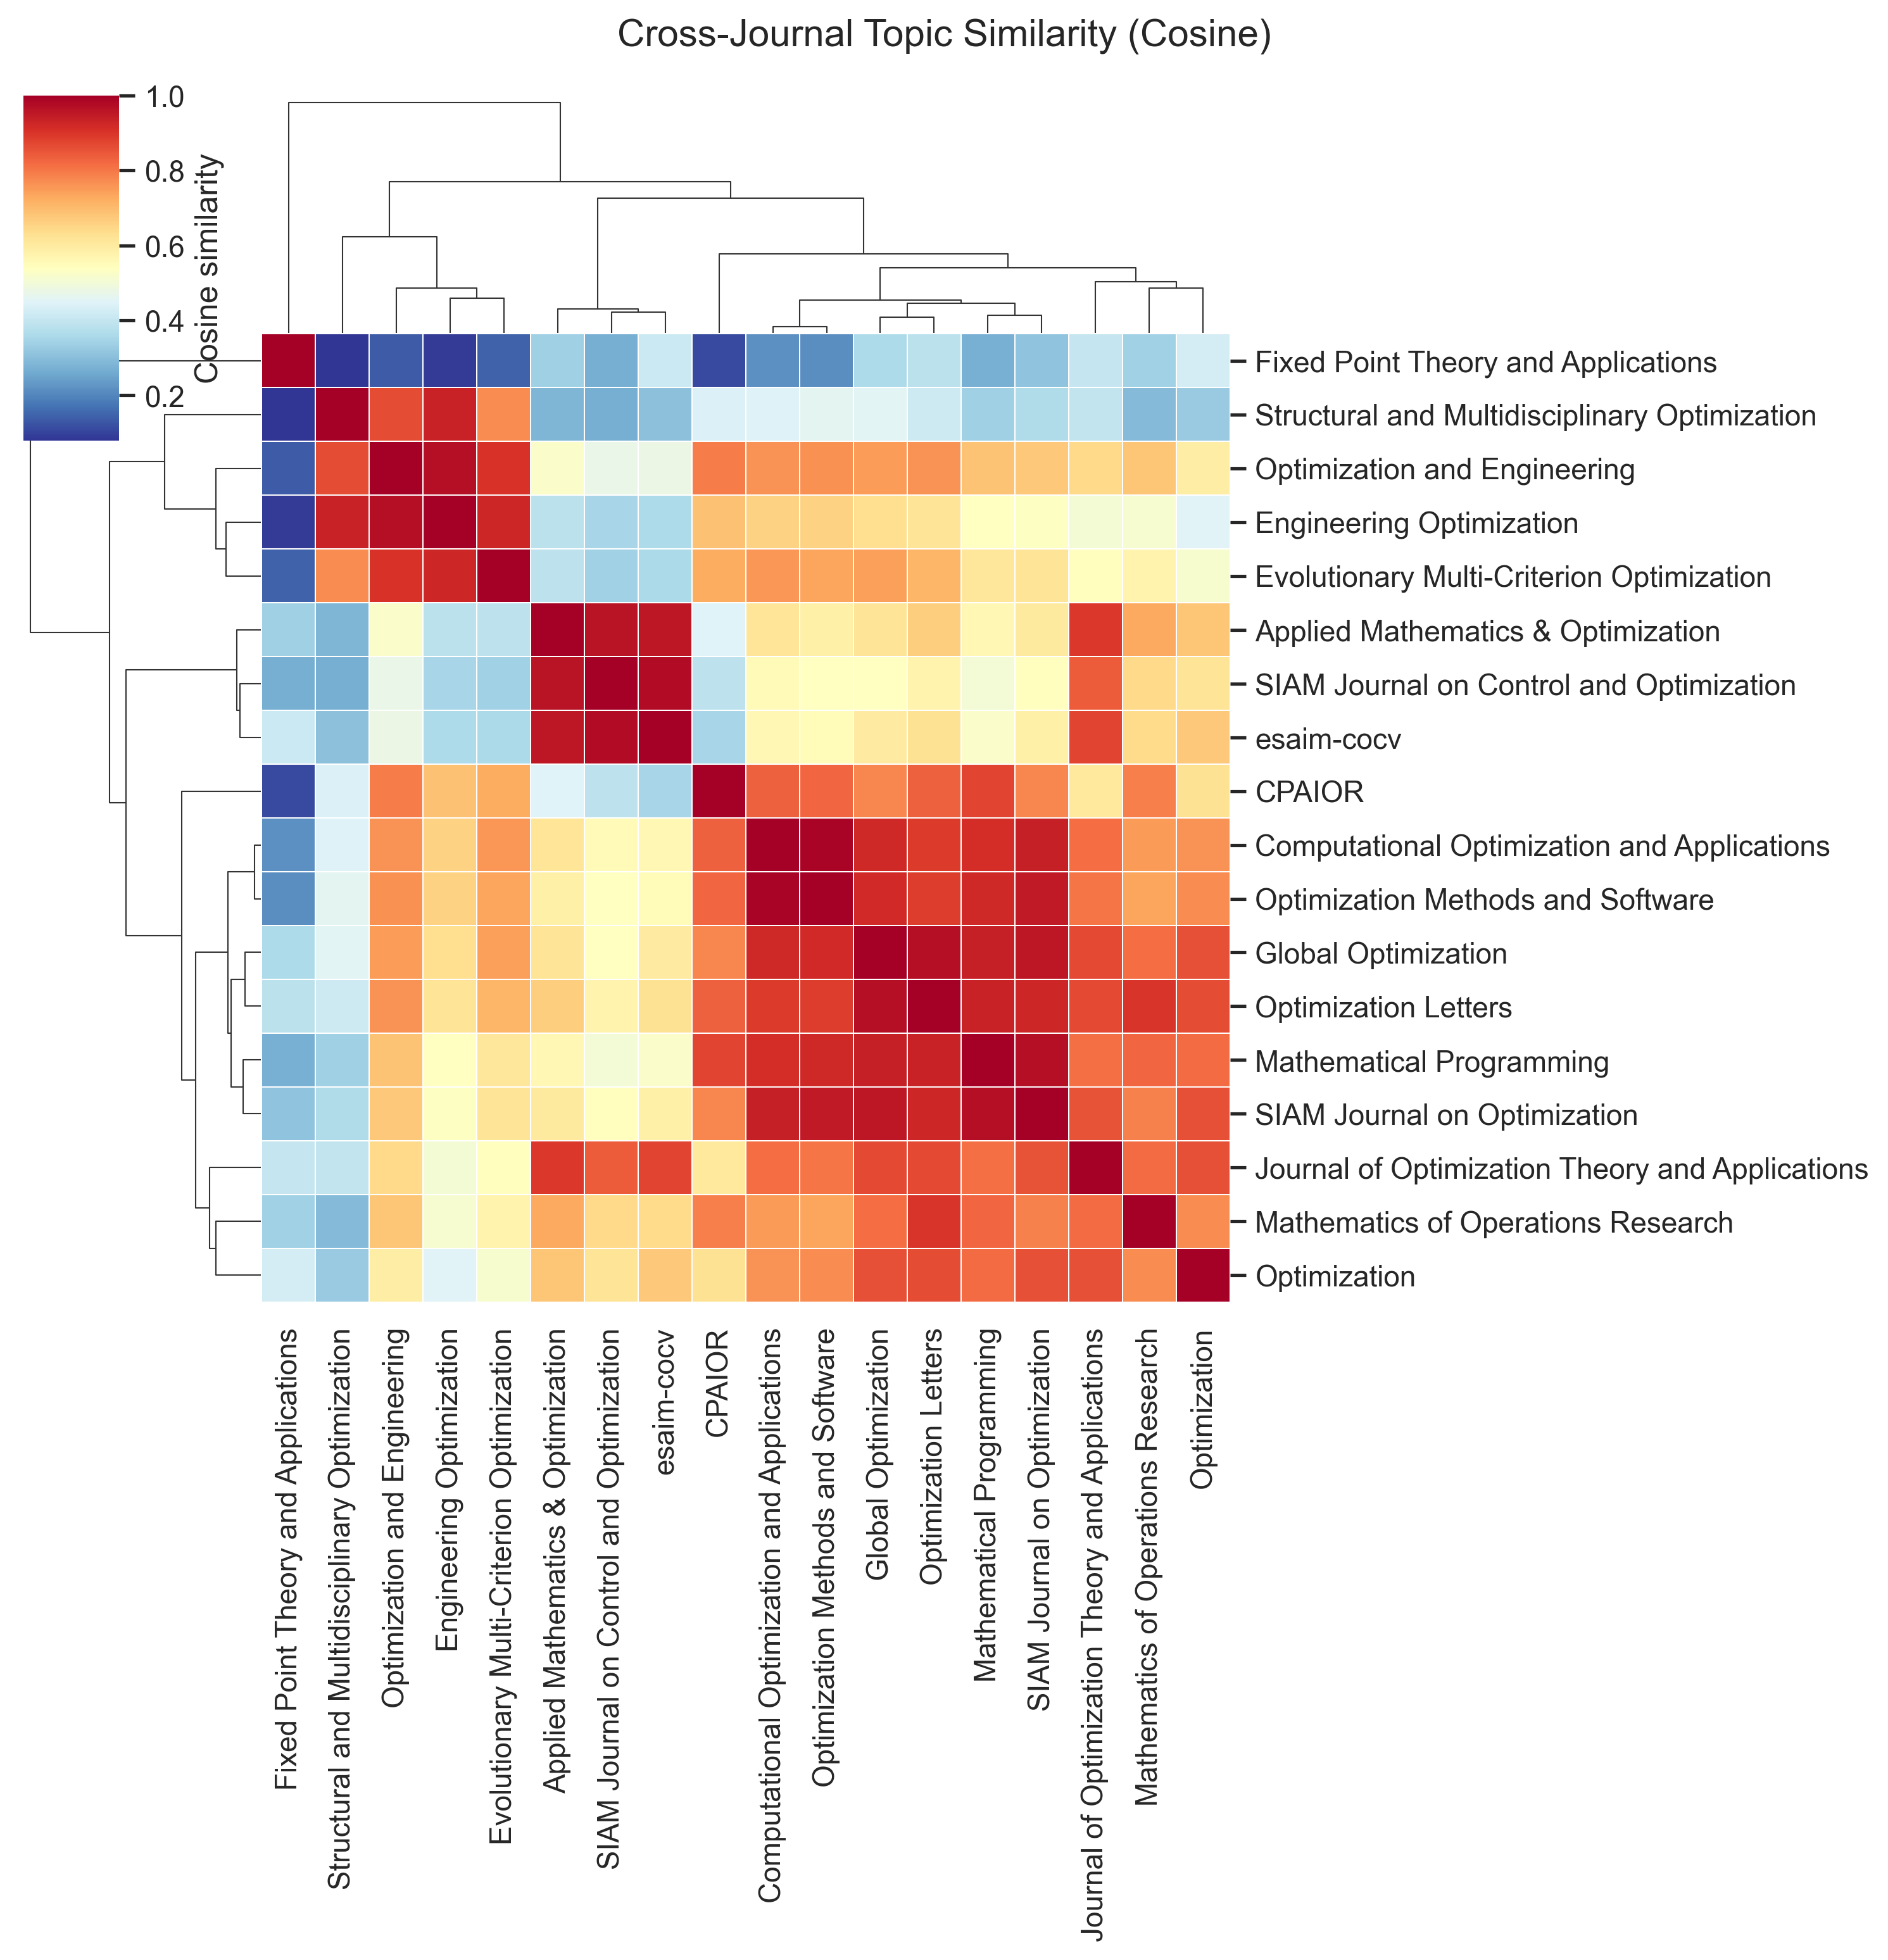
\includegraphics[width=\linewidth]{figures/journal_cosine_clustermap.png}
\caption{Hierarchical clustering of journals by cosine similarity of global topic profiles.}
\label{fig:clustermap}
\end{figure}

\begin{figure}[t]
\centering
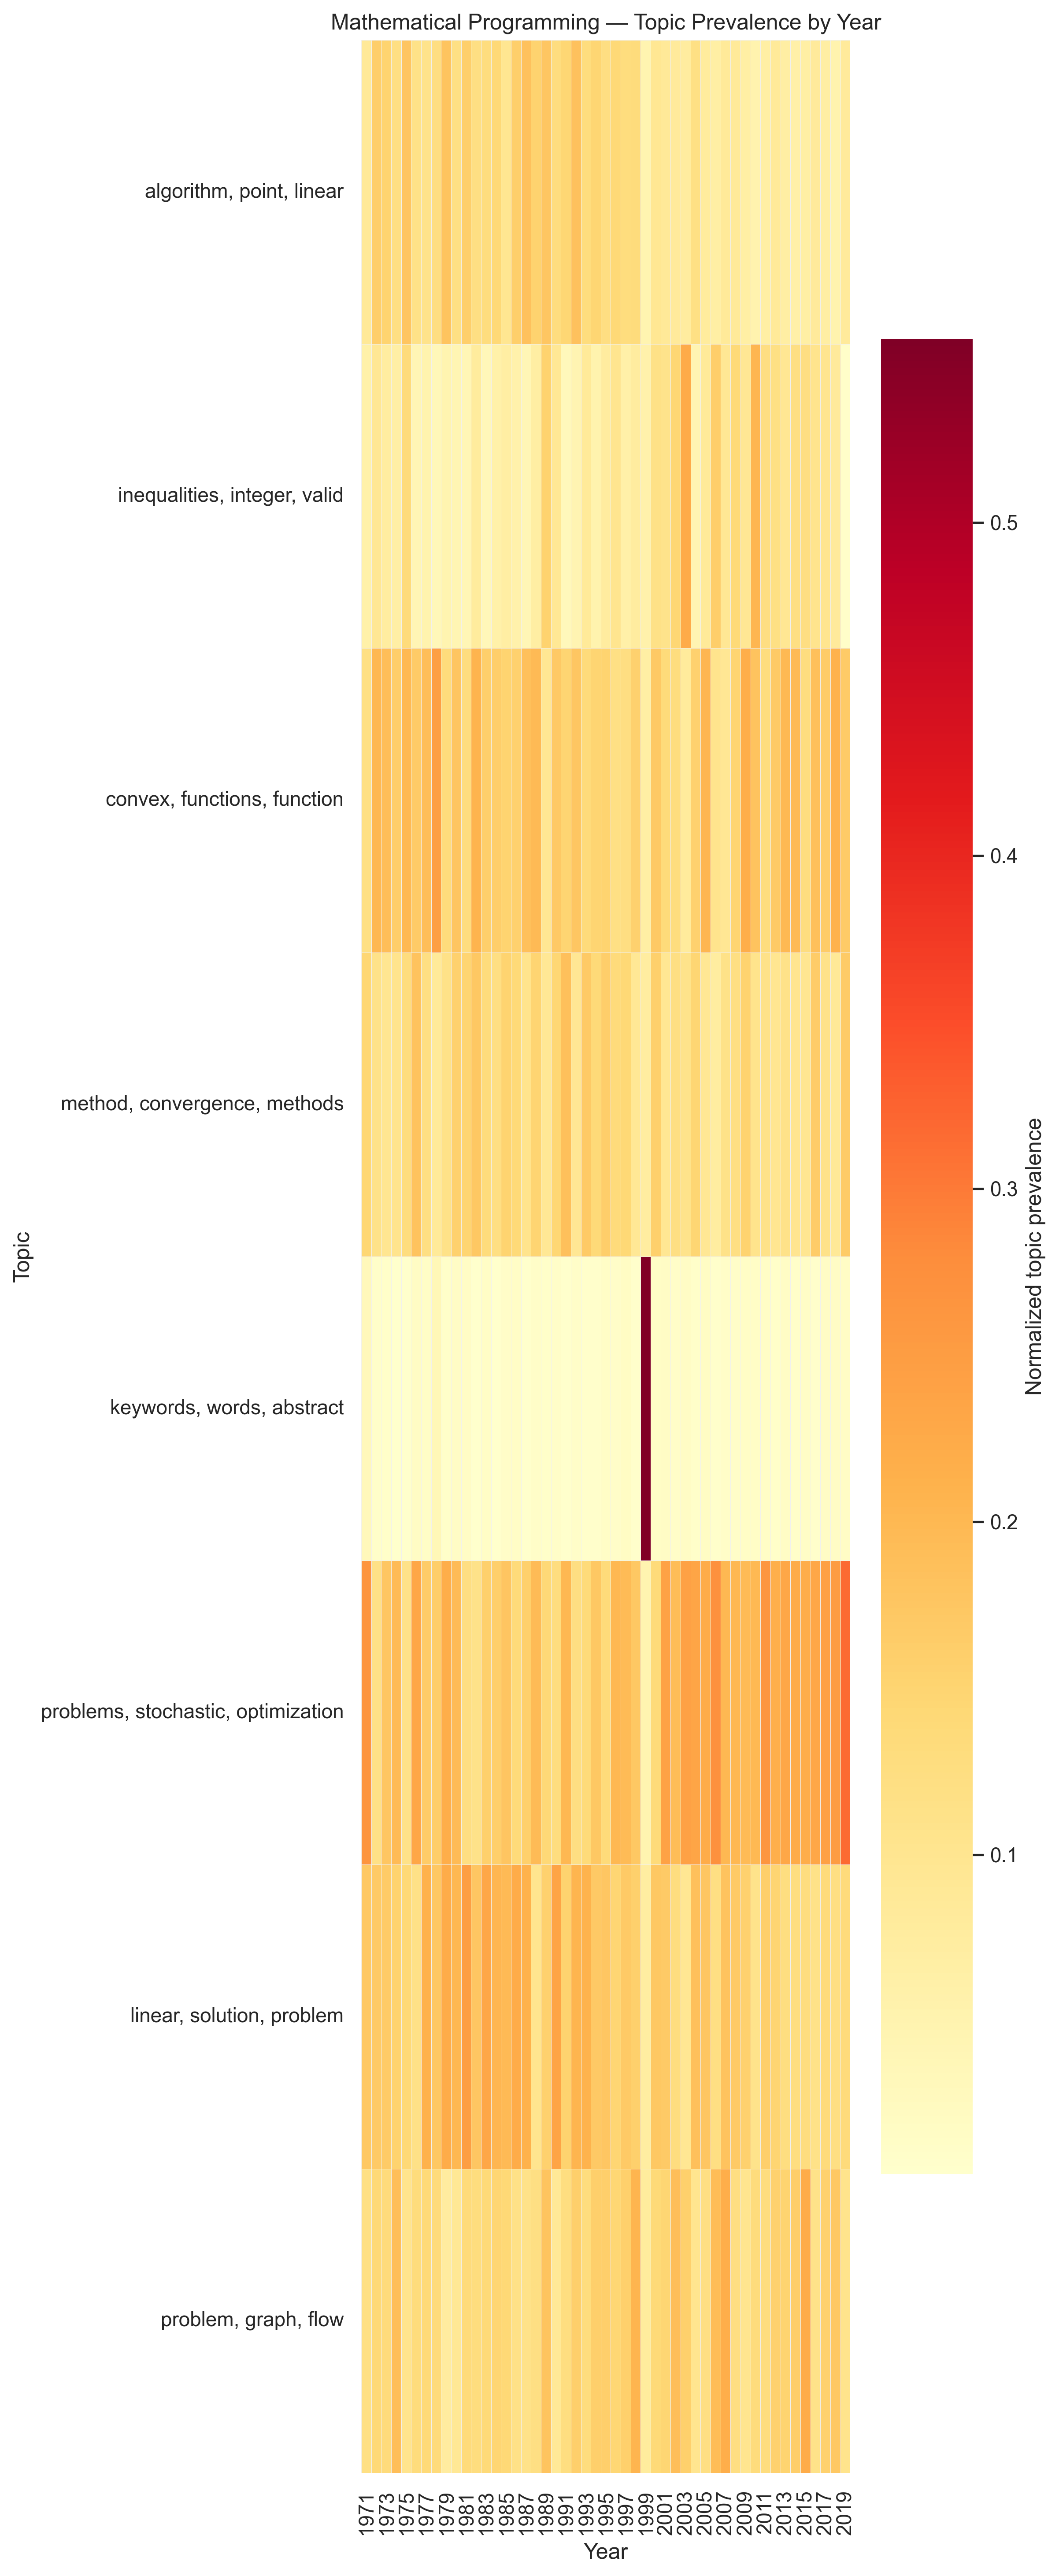
\includegraphics[width=\linewidth]{figures/mathematical_programming_topic_year_heatmap.png}
\caption{Temporal topic prevalence heatmap for \emph{Mathematical Programming}.}
\label{fig:mp_heatmap}
\end{figure}

\section{Applied Tasks: Journal Recommendation and Reviewer Matching}
\label{sec:applications}

OptLitBench supports two practical workflows using global topic vectors, implemented in \texttt{src/match\_manuscript.py}.

\subsection{Journal Recommendation}
Given a manuscript abstract $d^\star$, compute its TF-IDF vector under the global vectorizer, project to topic space via the global NMF model to obtain $h^\star$, and rank journals by cosine similarity $\cos(h^\star, p_j)$, where $p_j$ is the journal profile in Eq.~\eqref{eq:profile}.
This provides an evidence-based shortlist of venues aligned with the manuscript's latent themes.
In a CP/MIP scheduling example, \emph{Mathematical Programming} and \emph{CPAIOR} rank highest (cosine 0.638 and 0.615, respectively).

\subsection{Reviewer--Manuscript Matching}
Within a candidate journal $j$, rank existing publications by $\cos(h^\star, h_i)$ over $d_i\in\mathcal{D}_j$.
Top-$M$ matches suggest reviewers or related prior work most topically adjacent to the submission.
This is particularly useful when editorial boards seek reviewers for interdisciplinary optimization submissions.

Both tasks operate on released \texttt{global\_document\_topics.csv} and \texttt{journal\_topic\_profiles.csv} in the repository~\repo{}.

\section{Discussion and Limitations}
\label{sec:discussion}

\textbf{Visualization choice.} For scientometric papers, we recommend year $\times$ topic heatmaps as the primary figure type because they handle sparse monthly data and long time spans; smoothed line plots complement trend narration; monthly heatmaps are appropriate when publisher metadata includes month names (Springer sub-corpora).

\textbf{Limitations.}
(1) The benchmark is English-centric with standard English stopwords; multilingual abstracts are not explicitly modeled.
(2) Date extraction relies on directory naming conventions; metadata errors may affect temporal plots for a small fraction of records.
(3) NMF is a baseline; Poisson NMF~\cite{willis2021poisson} and embedding-based models~\cite{grootendorst2022bertopic} may improve coherence and cross-lingual robustness.
(4) Journal recommendation does not account for desk-reject policies, scope statements, or citation impact---topic similarity is necessary but not sufficient.
(5) Reviewer matching uses published abstracts as expertise proxies, not ground-truth reviewer assignments; empirical validation with editorial data is future work.

\textbf{Reproducibility.} Following applied data mining reproducibility practice, we release code, YAML configs, locked dependencies, evaluation CSVs, and 300-DPI figures at \repo{}.
The repository includes the OptLitBench corpus (\texttt{Data\_Abstract/}), all experiment outputs (\texttt{results/}), and scripts to regenerate reported artifacts.

\section{Conclusion}
\label{sec:conclusion}

We presented OptLitBench and a reproducible framework for temporal topic mining and cross-journal analytics on optimization literature.
The benchmark, metric suite, and applied matching protocols support applied data mining goals of novel datasets, comprehensive experimental analysis, and real-world scientometric utility.
Future work will extend the benchmark with topic coherence evaluation~\cite{roder2015coherence}, Poisson NMF baselines~\cite{willis2021poisson}, and validation against editorial metadata for recommendation tasks.

\section*{Acknowledgment}
This work was supported by the authors' affiliation with Criminal Investigation Police University of China.
We thank the publishers and communities whose publicly available bibliographic metadata made this benchmark possible.

\section*{Data and Code Availability}
OptLitBench is publicly available at \repo{}, including the abstract corpus, source code, configuration files, precomputed results, and figure assets used in this paper.

\bibliographystyle{IEEEtran}
\bibliography{references}

\end{document}
